\begin{SCn}

\scnsectionheader{\currentname}

\scnstartsubstruct

\scnheader{Предметная область Базового языка программирования ostis-систем (языка SCP -- Semantic Code Programming)}
\scntext{введение}{В качестве базового языка для описания программ обработки текстов
\textit{SC-кода} предлагается \textit{Язык SCP}.

\textit{Язык SCP} -- это графовый язык процедурного программирования,
предназначенный для эффективной обработки однородных семантических сетей
с теоретико-множественной интерпретацией, закодированных с помощью
\textit{SC-кода}. \textit{Язык SCP} является языком параллельного
асинхронного программирования.

Языком представления данных для текстов \textit{Языка SCP}
(\textit{scp-программ}) является \textit{SC-код} и, соответственно, любые
варианты его внешнего представления. \textit{Язык SCP} сам построен на
основе \textit{SC-кода}, вследствие чего \textit{scp-программы} сами по себе
могут входить в состав данных \textit{scp-программ}, в т.ч. по отношению к
самим себе. Таким образом, \textit{язык SCP} предоставляет возможность
построения реконфигурируемых программ. Однако для обеспечения
возможности реконфигурирования программы непосредственно в процессе ее
интерпретации необходимо на уровне интерпретатора \textit{Языка SCP
(Aбстрактной scp-машины)} обеспечить уникальность каждой исполняемой
копии исходной программы. Такую исполняемую копию, сгенерированную на
основе \textit{scp-программы}, будем называть \textit{scp-процессом}.
Включение знака некоторого \textit{действия в sc-памяти} во множество
\textit{scp-процессов} гарантирует тот факт, что в декомпозиции данного
действия будут присутствовать только знаки элементарных действий
(\textit{scp-операторов}), которые может интерпретировать реализация
\textit{Aбстрактной scp-машины}.

\textit{Язык SCP} рассматривается как ассемблер для графодинамического компьютера, ориентированного на хранение и обработку семантических сетей.

Таким образом, базовая модель обработки текстов \textit{SC-кода} включает в себя:

\begin{scnitemize}
\item
  Предметную область программ \textit{Языка SCP}, в которую включаются все тексты таких программ, в которой исследуется типология операторов этих  программ и заданные на них отношения.
\item
  Модель \textit{Абстрактной scp-машины}, т.е. интерпретатора \textit{scp-программ}, который должен являться частью \textit{платформы
  интерпретации sc-моделей компьютерных систем} (хотя в общем случае могут существовать варианты платформы, не содержащие такого интерпретатора, что, однако, не позволит использовать достоинства
  предлагаемой базовой модели).
\end{scnitemize}

Большинство достоинств базовой модели обработки текстов \textit{SC-кода}
имеют место благодаря двум основным ее особенностям:

\begin{scnitemize}
\item
  тексты программ \textit{Языка SCP} записываются при помощи тех же
  унифицированных семантических сетей, что и обрабатываемая информация;
\item
  подход к интерпретации \textit{scp-программ} предполагает создание при
  каждом вызове \textit{scp-программы} уникального \textit{scp-процесса}.
\end{scnitemize}

Перечислим эти достоинства:

\begin{scnitemize}
\item
  одновременно в общей памяти могут выполняться несколько независимых
  \textit{sc-агентов}, при этом разные копии \textit{sc-агентов} могут выполняться на разных
  серверах, за счет распределенной реализации интерпретатора sc-моделей
  (\textit{платформы реализации sc-моделей компьютерных систем}). Более
  того, \textit{Язык SCP} позволяет осуществлять параллельные асинхронные
  вызовы подпрограмм с последующей синхронизацией, и даже параллельно
  выполнять операторы в рамках одной \textit{scp-программы};
\item
  перенос \textit{sc-агента} из одной системы в другую заключается в простом
  переносе фрагмента базы знаний, без каких-либо дополнительных
  операций, зависящих от платформы интерпретации;
\item
  тот факт, что спецификации \textit{sc-агентов} и их программы могут быть записаны
  на том же языке, что и обрабатываемые знания, существенно сокращает
  перечень специализированных средств, предназначенных для
  проектирования машин обработки знаний, и упрощает их разработку за
  счет использования более универсальных компонентов;
\item
  тот факт, что для интерпретации \textit{scp-программы} создается
  соответствующий ей уникальный \textit{scp-процесс}, позволяет по
  возможности оптимизировать план выполнения перед его реализацией и
  даже непосредственно в процессе выполнения без потенциальной опасности
  испортить общий универсальный алгоритм всей программы. Более того,
  такой подход к проектированию и интерпретации программ позволяет
  говорить о возможности создания \textit{самореконфигурируемых программ};
  
\end{scnitemize}

}

\scniselement{предметная область}
\scnsdmainclasssingle{scp-программа}
\scnsdclass{агентная scp-программа;scp-процесс;scp-оператор;атомарный тип scp-оператора}
\scnsdrelation{начальный оператор';параметр scp-программы';in-параметр’;out-параметр’;scp-операнд’}

\scnheader{scp-программа}
\scnidtf{Язык SCP}
\scnrelto{включение}{программа в sc-памяти}
\scnexplanation{Каждая \textbf{\textit{scp-программа}} представляет собой \textit{обобщенную структуру}, описывающую один из вариантов декомпозиции действий некоторого класса, выполняемых в sc-памяти. Знак \textit{sc-переменной}, соответствующей конкретному декомпозируемому действию является в рамках \textbf{\textit{scp-программы}} \textit{ключевым sc-элементом'}. Также явно указывается принадлежность данного знака множеству \textit{scp-процессов}.

Таким образом, каждая \textbf{\textit{scp-программа}} описывает в обобщенном виде декомпозицию некоторого \textit{scp-процесса} на взаимосвязанные \textit{scp-операторы}, с указанием, при их наличии, аргументов для данного \textit{scp-процесса}.

По сути каждая \textbf{\textit{scp-программа}} представляет собой описание последовательности элементарных операций, которые необходимо выполнить над семантической сетью, чтобы выполнить более сложное действие некоторого класса.}
\scnrelfrom{типичная семантическая окрестность}{
\scnfilelong{
\begin{figure}[H]
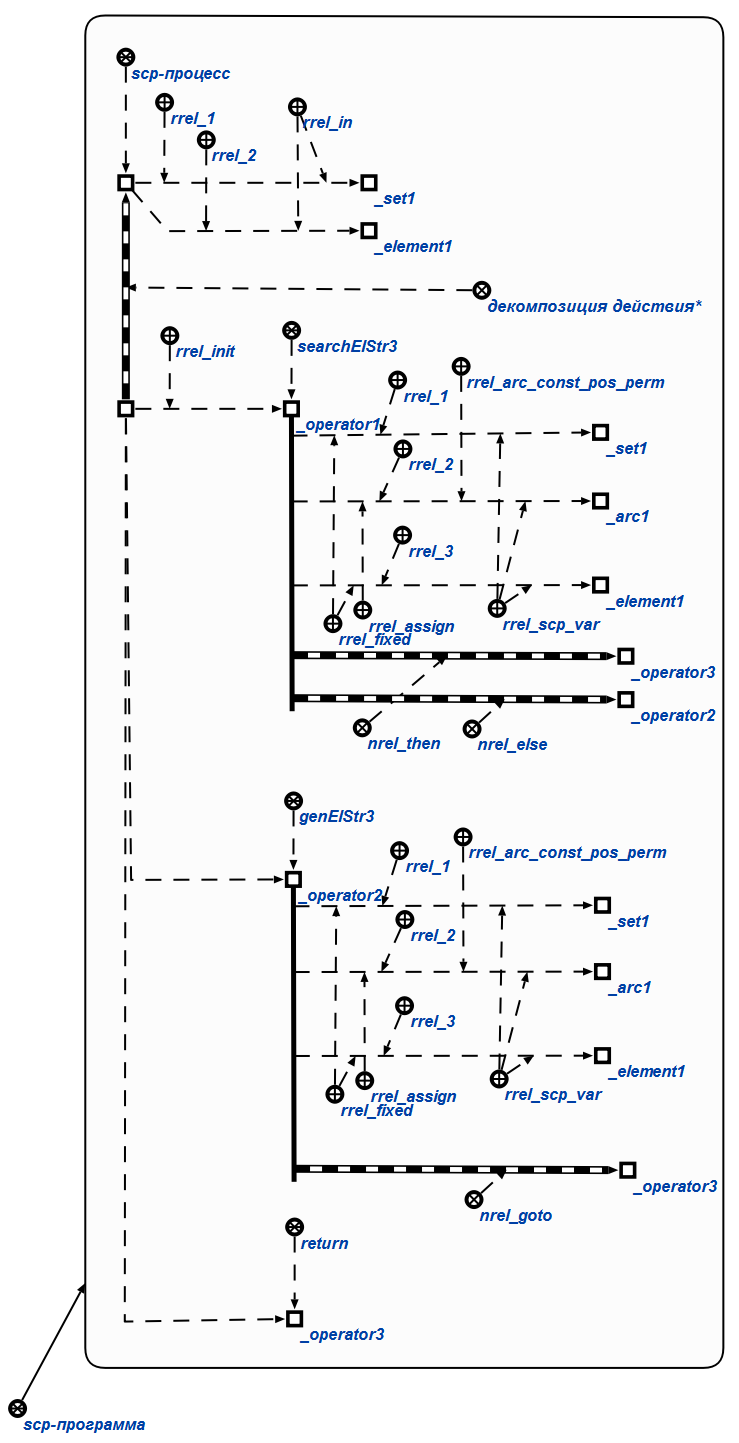
\includegraphics[width=0.8\linewidth]{figures/sd_scp/examplescp1.png}
\end{figure}
}}
\scnaddlevel{1}
\scnexplanation{В приведенном примере показана \textit{scp-программа}, состоящая из трех \textit{scp-операторов}. Данная программа проверяет, содержится ли в заданном множестве (первый параметр) заданный элемент (второй параметр), и, если нет, то добавляет его в это множество.}
\scnaddlevel{-1}

\scnheader{агентная scp-программа}
\scnrelto{включение}{scp-программа}
\scnexplanation{\textbf{\textit{агентные scp-программы}} представляют собой частный случай \textit{scp-программ} вообще, однако заслуживают отдельного рассмотрения, поскольку используются наиболее часто. \textit{scp-программы} данного класса представляют собой реализации программ агентов обработки знаний, и имеют жестко фиксированный набор параметров. Каждая такая программа имеет ровно два \textit{in-параметра’}. Значение первого параметра является знаком бинарной ориентированной пары, являющейся вторым компонентом связки отношения \textit{первичное условие инициирования*} для абстрактного \textit{sc-агента}, в множество \textit{программ sc-агента*} которого входит рассматриваемая \textbf{\textit{агентная scp-программа}}, и, по сути, описывает класс событий, на которые реагирует указанный sc-агент.

Значением второго параметра является \textit{sc-элемент}, с которым непосредственно связано событие, в результате возникновения которого был инициирован соответствующий \textit{sc-агент}, т.е., например, сгенерированная либо удаляемая \textit{sc-дуга} или \textit{sc-ребро}.}

\scnheader{абстрактный sc-агент, реализуемый на Языке SCP}
\scnexplanation{Для sc-агентов, программы которых реализованы с использованием
\textit{Языка SCP}, справедливы общие принципы организации взаимодействия
\textit{sc-агентов} и пользователей \textit{ostis-системы} через общую
\textit{sc-память.}

Помимо общих принципов для \textit{sc-агентов}, реализованных с использованием \textit{Языка SCP}, вводятся следующие дополнительные уточнения:

\begin{scnitemize}
\item
  
  В результате появления в sc-памяти некоторой конструкции,
  удовлетворяющей условию инициирования какого-либо \textit{абстрактного
  sc-агента}, реализованного при помощи \textit{Языка SCP}, в
  \textit{sc-памяти} генерируется и инициируется \textit{scp-процесс}. В
  качестве шаблона для генерации используется \textit{агентная
  scp-программа}, указанная во множестве программ соответствующего
  \textit{абстрактного sc-агента}.
  
\item
  
  Каждый такой \textit{scp-процесс}, соответствующий некоторой
  \textit{агентной scp-программе}, может быть связан с набором структур,
  описывающих блокировки различных типов. Таким образом, синхронизация
  взаимодействия параллельно выполняемых \textit{scp-процесcов}
  осуществляется так же, как и в случае любых других \textit{действий в
  sc-памяти};
  
\item
  
  В рамках \textit{scp-процесса} могут создаваться дочерние
  \textit{scp-процессы}, однако синхронизация между ними при необходимости
  осуществляется посредством введения дополнительных внутренних
  блокировок. Таким образом, каждый \textit{scp-процесс} с точки зрения
  \textit{процессов в sc-памяти} является атомарным и законченным актом
  деятельности некоторого \textit{sc-агента}.
  
\item
  
  Во избежание нежелательных изменений в самом теле \textit{scp-процесса},
  вся конструкция, сгенерированная на основе некоторой
  \textit{scp-программы} (весь текст \textit{scp-процесса}), должна быть
  добавлена в \textit{полную блокировку}, соответствующую данному \textit{scp-процессу}.
  
\item
  Все конструкции, сгенерированные в процессе выполнения
  \textit{scp-процесса}, автоматически попадают в \textit{полную
  блокировку}, соответствующую данному \textit{scp-процессу}.
  Дополнительно следует отметить, что знак самой этой структуры и вся метаинформация о ней также включаются в эту структуру.
\item
  При необходимости можно вручную разблокировать или заблокировать   некоторую конструкцию каким-либо типом блокировки, используя   соответствующие \textit{scp-операторы} класса \textit{scp-оператор управления
  блокировками}.
\item
  После завершения выполнения некоторого \textit{scp-процесса} его текст как
  правило, удаляется из \textit{sc-памяти}, а все заблокированные
  конструкции освобождаются (разрушаются знаки структур, обозначавших
  блокировки).
\item
  Несмотря на то, что каждый \textit{scp-оператор} представляет собой атомарное
 \textit{действие в sc-памяти}, дополнительные блокировки, соответствующие
  одному оператору не вводятся, чтобы избежать громоздкости и избытка
  дополнительных системных конструкций, создаваемых при выполнении
  некоторого \textit{scp-процесса}. Вместо этого используются блокировки, общие
  для всего \textit{scp-процесса}. Таким образом, агенты \textit{Абстрактной scp-машины}
  при интерпретации \textit{scp-операторов} работают только с учетом блокировок,
  общих для всего интерпретируемого \textit{scp-процесса}.
\item
  Как правило, частный \textit{класс действий}, соответствующий конкретной
  \textit{scp-программе} явно не вводится, а используется более общий
  класс \textit{scp-процесс}, за исключением тех случаев, когда введение
  специального \textit{класса действий} необходимо по каким-либо другим
  соображениям.
\end{scnitemize}}

\scnheader{scp-процесс}
\scnexplanation{Под \textbf{\textit{scp-процессом}} понимается некоторое \textit{действие в sc-памяти}, однозначно описывающее конкретный акт выполнения некоторой \textit{scp-программы} для заданных исходных данных. Если \textit{scp-программа} описывает алгоритм решения какой-либо задачи в общем виде, то \textit{scp-процесс} обозначает конкретное действие, реализующее данный алгоритм для заданных входных параметров.

По сути, \textbf{\textit{scp-процесс}} представляет собой уникальную копию, созданную на основе \textit{scp-программы}, в которой каждой \textit{sc-переменной}, за исключением \textit{scp-переменных'}, соответствует сгенерированная \textit{sc-константа}.

Принадлежность некоторого действия множеству \textit{scp-процессов} гарантирует тот факт, что в декомпозиции данного действия будут присутствовать только знаки элементарных действий (\textit{scp-операторов}), которые может интерпретировать реализация \textit{Абстрактной scp-машины}.}
\scnrelfrom{пример выполнения}{
\scnfilelong{
\begin{figure}[H]
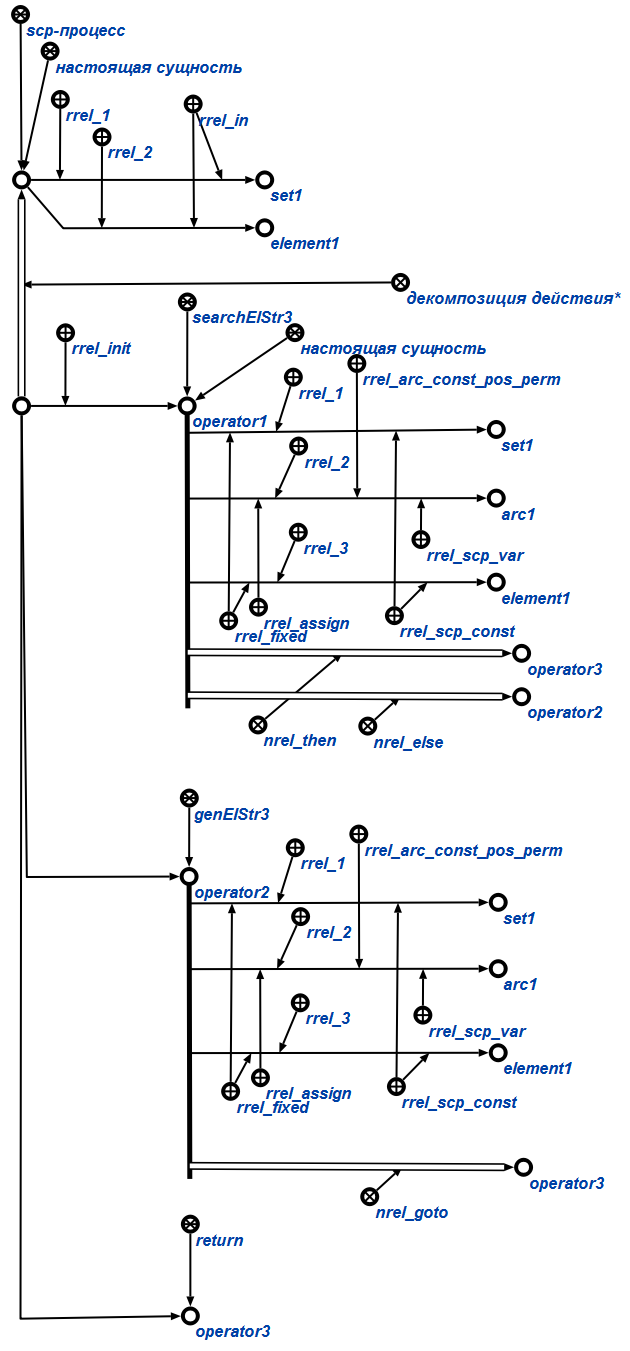
\includegraphics[width=0.6\linewidth]{figures/sd_scp/examplescp2.png}
\end{figure}
\begin{figure}[H]
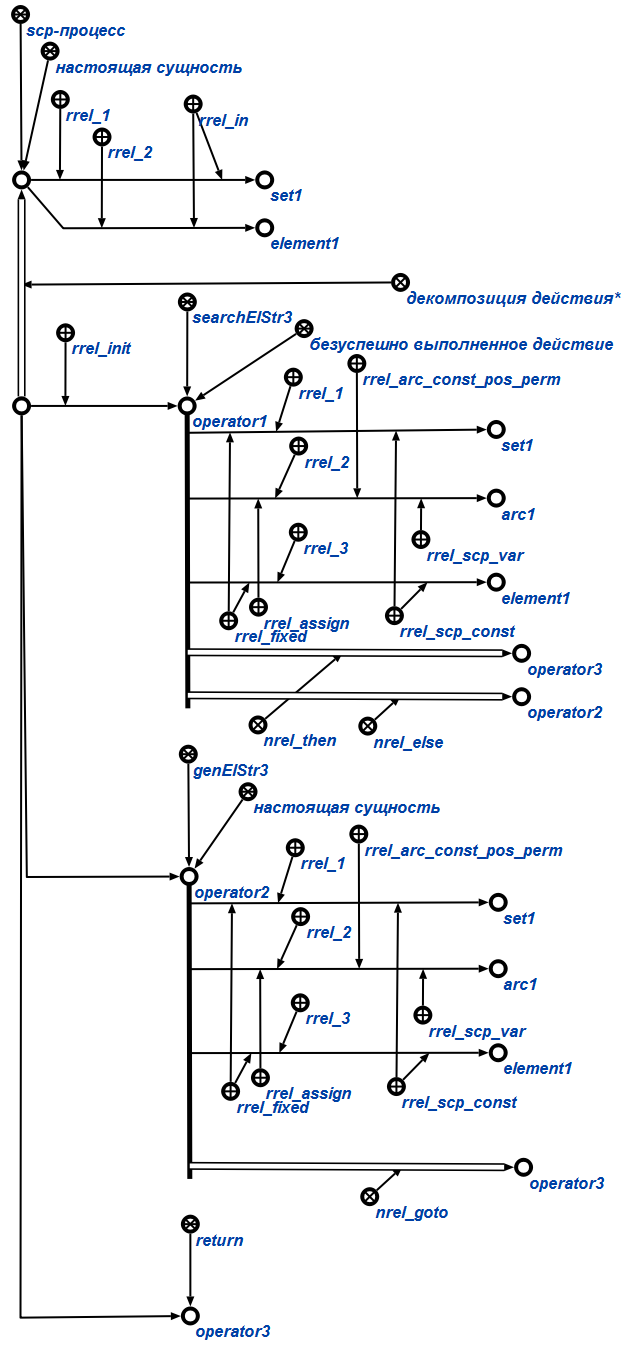
\includegraphics[width=0.6\linewidth]{figures/sd_scp/examplescp3.png}
\end{figure}
\begin{figure}[H]
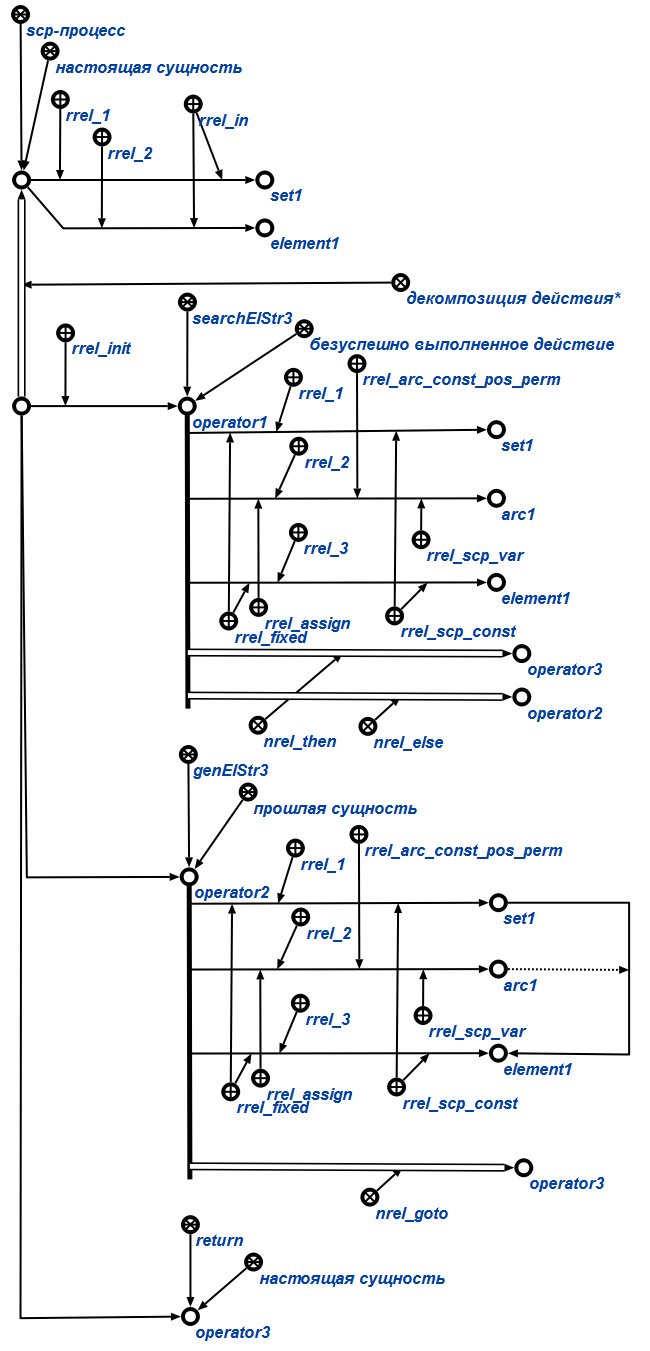
\includegraphics[width=0.6\linewidth]{figures/sd_scp/examplescp4.png}
\end{figure}
\begin{figure}[H]
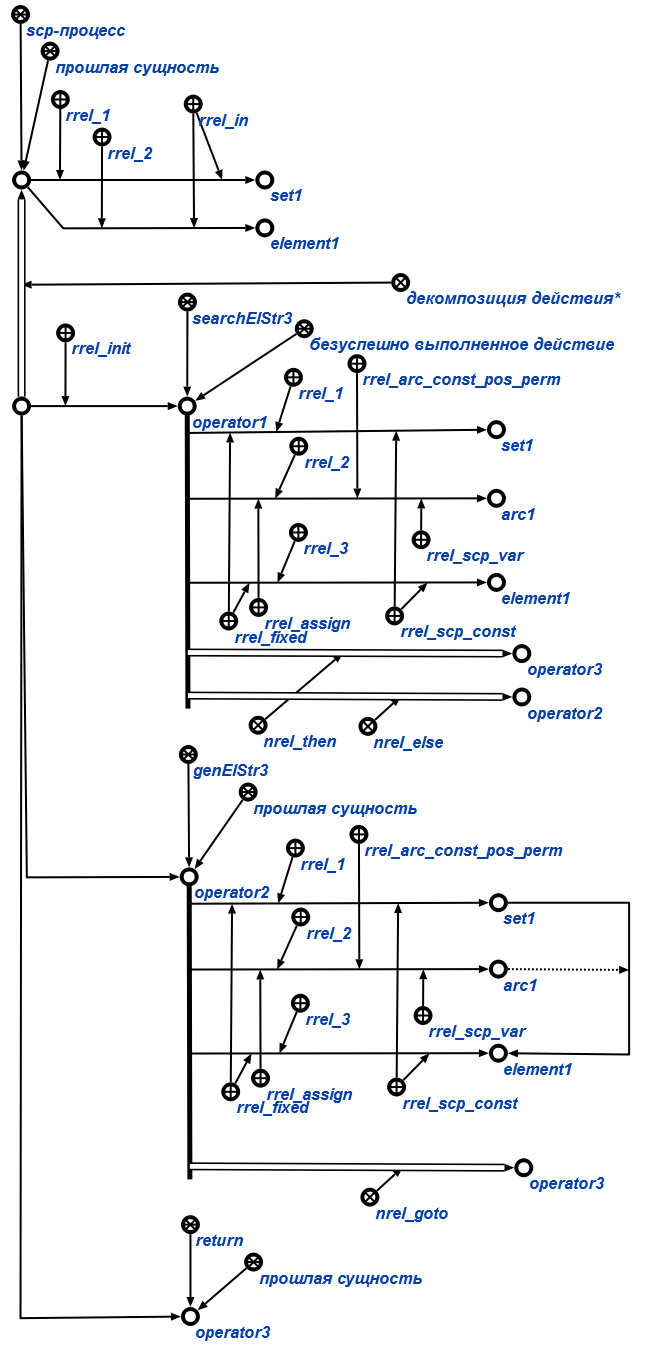
\includegraphics[width=0.6\linewidth]{figures/sd_scp/examplescp5.png}
\end{figure}
}}
\scnaddlevel{1}
\scnexplanation{В приведенном примере последовательно показаны состояния scp-процесса, соответствующего scp-программе, добавляющей заданный элемент в заданное множество, если он там ранее не содержался. В примере предполагается, что рассматриваемый элемент (element1) изначально не содержится во множестве (set1).}
\scnaddlevel{-1}

\scnheader{scp-оператор}
\scnrelto{включение}{действие в sc-памяти}
\scnrelto{семейство подмножеств}{атомарный тип scp-оператора}
\scnexplanation{Каждый \textbf{\textit{scp-оператор}} представляет собой некоторое элементарное \textit{действие в sc-памяти}. Аргументы \textit{scp-оператора} будем называть операндами. Порядок операндов указывается при помощи соответствующих ролевых отношений (\textit{1’}, \textit{2’}, \textit{3’} и так далее). Операнд, помеченный ролевым отношением \textit{1’}, будем называть первым операндом и т.д., помеченный ролевым отношением \textit{2’} – вторым операндом, и т.д. Тип и смысл каждого операнда также уточняется при помощи различных подклассов отношения \textit{scp-операнд'}. В общем случае операндом может быть любой \textit{sc-элемент}, в том числе, знак какой-либо \textit{scp-программы}, в том числе самой программы, содержащей данный оператор.

Каждый \textbf{\textit{scp-оператор}} должен иметь один и более операнд, а также указание того \textbf{\textit{scp-оператора}} (или нескольких), который должен быть выполнен следующим. Исключение их данного правила составляет \textit{scp-оператор завершения выполнения программы}, который не содержит ни одного операнда и после выполнения которого никакие \textit{scp-операторы} в рамках данной программы выполняться не могут.}

\scnheader{атомарный тип scp-оператора}
\scnexplanation{Каждый \textbf{\textit{атомарный тип scp-оператора}} представляет собой класс \textit{scp-операторов}, который не разбивается на более частные, и, соответственно, интерпретируется реализацией \textit{Aбстрактной scp-машины}.}

\scnheader{начальный оператор'}
\scnrelto{включение}{1'}
\scnexplanation{Ролевое отношение \textbf{\textit{начальный оператор'}} указывает в рамках декомпозиции соответствующего \textit{scp-программе} \textit{scp-процесса} те \textit{scp-операторы}, которые должны быть выполнены в первую очередь, т.е. те, с которых собственно начинается выполнение \textit{scp-процесса}.}

\scnheader{параметр scp-программы'}
\scnrelto{включение}{аргумент действия'}
\scnsubdividing{in-параметр’;out-параметр’}
\scnexplanation{Ролевое отношение \textbf{\textit{параметр scp-программы'}} связывает знак соответствующего \textit{scp-программе} \textit{scp-процесса} с его аргументами.}

\scnheader{in-параметр’}
\scnexplanation{Параметры типа \textbf{\textit{in-параметр'}} хоть и соответствуют \textit{переменным scp-программы’}, не могут менять значение в процессе ее интерпретации. Фиксированное значение переменной устанавливается при создании уникальной копии \textit{scp-программы} (\textit{scp-процесса}) для ее интерпретации, и, таким образом, соответствующая \textit{scp-переменная'} на момент начала ее интерпретации становится \textit{scp-константой'} в рамках каждого \textit{scp-оператора}, в котором встречалась данная \textit{scp-переменная'}. Использование \textit{in-параметров} можно рассматривать по аналогии с использованием варианта механизма передачи по значению в традиционных языках программирования, с тем условием, что значение локальной переменной в рамках дочерней программы не может быть изменено.}

\scnheader{out-параметр’}
\scnexplanation{Параметры типа \textbf{\textit{out-параметр'}} соответствуют \textit{переменным scp-программы'} и обладают всеми теми же соответствующими свойствами. Чаще всего предполагается, что значение данного параметра необходимо родительской \textit{scp-программе}, содержащей оператор вызова текущей \textit{scp-программы}. При этом на момент начала интерпретации в качестве параметра дочернему процессу передается непосредственно узел, обозначающий переменную (а точнее, ее уникальную копию в рамках процесса) родительского процесса. Указанная переменная может при необходимости иметь значение, либо не иметь. После завершения и во время интерпретации дочернего процесса родительский процесс по-прежнему может работать с переменной, переданной в качестве \textit{out-параметра'}, при необходимости просматривая или изменяя ее значение. Использование out-параметра можно рассматривать по аналогии с использованием механизма передачи по ссылке в традиционных языках программирования.}

\scnheader{scp-операнд’}
\scnrelto{включение}{аргумент действия'}
\scniselement{неосновное понятие}
\scniselement{ролевое отношение}
\scnexplanation{Ролевое отношение \textbf{\textit{scp-операнд’}} является неосновным понятием и указывает на принадлежность аргументов \textit{scp-оператору}. Помимо указания какого-либо класса \textbf{\textit{scp-операндов’}} порядок аргументов \textit{scp-оператора} дополнительно уточняется \textit{ролевыми отношениями 1'}, \textit{2'} и т.д.}

\scnendstruct

\end{SCn}
